\documentclass[twoside]{book}

% Packages required by doxygen
\usepackage{fixltx2e}
\usepackage{calc}
\usepackage{doxygen}
\usepackage[export]{adjustbox} % also loads graphicx
\usepackage{graphicx}
\usepackage[utf8]{inputenc}
\usepackage{makeidx}
\usepackage{multicol}
\usepackage{multirow}
\PassOptionsToPackage{warn}{textcomp}
\usepackage{textcomp}
\usepackage[nointegrals]{wasysym}
\usepackage[table]{xcolor}

% Font selection
\usepackage[T1]{fontenc}
\usepackage[scaled=.90]{helvet}
\usepackage{courier}
\usepackage{amssymb}
\usepackage{sectsty}
\renewcommand{\familydefault}{\sfdefault}
\allsectionsfont{%
  \fontseries{bc}\selectfont%
  \color{darkgray}%
}
\renewcommand{\DoxyLabelFont}{%
  \fontseries{bc}\selectfont%
  \color{darkgray}%
}
\newcommand{\+}{\discretionary{\mbox{\scriptsize$\hookleftarrow$}}{}{}}

% Page & text layout
\usepackage{geometry}
\geometry{%
  a4paper,%
  top=2.5cm,%
  bottom=2.5cm,%
  left=2.5cm,%
  right=2.5cm%
}
\tolerance=750
\hfuzz=15pt
\hbadness=750
\setlength{\emergencystretch}{15pt}
\setlength{\parindent}{0cm}
\setlength{\parskip}{3ex plus 2ex minus 2ex}
\makeatletter
\renewcommand{\paragraph}{%
  \@startsection{paragraph}{4}{0ex}{-1.0ex}{1.0ex}{%
    \normalfont\normalsize\bfseries\SS@parafont%
  }%
}
\renewcommand{\subparagraph}{%
  \@startsection{subparagraph}{5}{0ex}{-1.0ex}{1.0ex}{%
    \normalfont\normalsize\bfseries\SS@subparafont%
  }%
}
\makeatother

% Headers & footers
\usepackage{fancyhdr}
\pagestyle{fancyplain}
\fancyhead[LE]{\fancyplain{}{\bfseries\thepage}}
\fancyhead[CE]{\fancyplain{}{}}
\fancyhead[RE]{\fancyplain{}{\bfseries\leftmark}}
\fancyhead[LO]{\fancyplain{}{\bfseries\rightmark}}
\fancyhead[CO]{\fancyplain{}{}}
\fancyhead[RO]{\fancyplain{}{\bfseries\thepage}}
\fancyfoot[LE]{\fancyplain{}{}}
\fancyfoot[CE]{\fancyplain{}{}}
\fancyfoot[RE]{\fancyplain{}{\bfseries\scriptsize Generated by Doxygen }}
\fancyfoot[LO]{\fancyplain{}{\bfseries\scriptsize Generated by Doxygen }}
\fancyfoot[CO]{\fancyplain{}{}}
\fancyfoot[RO]{\fancyplain{}{}}
\renewcommand{\footrulewidth}{0.4pt}
\renewcommand{\chaptermark}[1]{%
  \markboth{#1}{}%
}
\renewcommand{\sectionmark}[1]{%
  \markright{\thesection\ #1}%
}

% Indices & bibliography
\usepackage{natbib}
\usepackage[titles]{tocloft}
\setcounter{tocdepth}{3}
\setcounter{secnumdepth}{5}
\makeindex

% Hyperlinks (required, but should be loaded last)
\usepackage{ifpdf}
\ifpdf
  \usepackage[pdftex,pagebackref=true]{hyperref}
\else
  \usepackage[ps2pdf,pagebackref=true]{hyperref}
\fi
\hypersetup{%
  colorlinks=true,%
  linkcolor=blue,%
  citecolor=blue,%
  unicode%
}

% Custom commands
\newcommand{\clearemptydoublepage}{%
  \newpage{\pagestyle{empty}\cleardoublepage}%
}

\usepackage{caption}
\captionsetup{labelsep=space,justification=centering,font={bf},singlelinecheck=off,skip=4pt,position=top}

%===== C O N T E N T S =====

\begin{document}

% Titlepage & ToC
\hypersetup{pageanchor=false,
             bookmarksnumbered=true,
             pdfencoding=unicode
            }
\pagenumbering{alph}
\begin{titlepage}
\vspace*{7cm}
\begin{center}%
{\Large My Project }\\
\vspace*{1cm}
{\large Generated by Doxygen 1.8.13}\\
\end{center}
\end{titlepage}
\clearemptydoublepage
\pagenumbering{roman}
\tableofcontents
\clearemptydoublepage
\pagenumbering{arabic}
\hypersetup{pageanchor=true}

%--- Begin generated contents ---
\chapter{Project title}
\label{index}\hypertarget{index}{}This is the main page for the project.


\begin{DoxyEnumerate}
\item item 1
\item item 2
\item item 3
\item item 4 
\end{DoxyEnumerate}
\chapter{Page 1}
\label{Page_1}
\Hypertarget{Page_1}
\hyperlink{Subpage_1}{Sub Page 1}

{\bfseries Author\+:} Author name {\bfseries Date\+:} Date \subsection*{Module\textquotesingle{}s Role}

Explain the module\textquotesingle{}s role in the system in general \hypertarget{Subpage_1}{}\section{Sub Page 1}\label{Subpage_1}
{\bfseries Author\+:} Yanhua Feng {\bfseries Date\+:} 09.\+07.\+2020 \subsection*{Module\textquotesingle{}s Role}

Explain the module\textquotesingle{}s role in the system in general 
\chapter{Page 2}
\label{Page_2}
\Hypertarget{Page_2}
{\bfseries Author\+:} Lin Chen {\bfseries Date\+:} 09.\+07.\+2020 \subsection*{Module\textquotesingle{}s Role}

Explain the module\textquotesingle{}s role in the system in general 
\chapter{File Index}
\section{File List}
Here is a list of all documented files with brief descriptions\+:\begin{DoxyCompactList}
\item\contentsline{section}{/home/lin\+\_\+chen/\+C\+S3335/\+Doxygen/\+P6/include/\hyperlink{hello_8h}{hello.\+h} }{\pageref{hello_8h}}{}
\item\contentsline{section}{/home/lin\+\_\+chen/\+C\+S3335/\+Doxygen/\+P6/include/{\bfseries test\+\_\+1.\+h} }{\pageref{test__1_8h}}{}
\item\contentsline{section}{/home/lin\+\_\+chen/\+C\+S3335/\+Doxygen/\+P6/include/{\bfseries test\+\_\+2.\+h} }{\pageref{test__2_8h}}{}
\item\contentsline{section}{/home/lin\+\_\+chen/\+C\+S3335/\+Doxygen/\+P6/include/\hyperlink{util_8h}{util.\+h} }{\pageref{util_8h}}{}
\item\contentsline{section}{/home/lin\+\_\+chen/\+C\+S3335/\+Doxygen/\+P6/src/\hyperlink{hello_8c}{hello.\+c} }{\pageref{hello_8c}}{}
\item\contentsline{section}{/home/lin\+\_\+chen/\+C\+S3335/\+Doxygen/\+P6/src/\hyperlink{main_8c}{main.\+c} }{\pageref{main_8c}}{}
\item\contentsline{section}{/home/lin\+\_\+chen/\+C\+S3335/\+Doxygen/\+P6/src/\hyperlink{util_8c}{util.\+c} }{\pageref{util_8c}}{}
\end{DoxyCompactList}

\chapter{File Documentation}
\hypertarget{hello_8h}{}\section{/home/lin\+\_\+chen/\+C\+S3335/\+Doxygen/\+P6/include/hello.h File Reference}
\label{hello_8h}\index{/home/lin\+\_\+chen/\+C\+S3335/\+Doxygen/\+P6/include/hello.\+h@{/home/lin\+\_\+chen/\+C\+S3335/\+Doxygen/\+P6/include/hello.\+h}}
This graph shows which files directly or indirectly include this file\+:\nopagebreak
\begin{figure}[H]
\begin{center}
\leavevmode
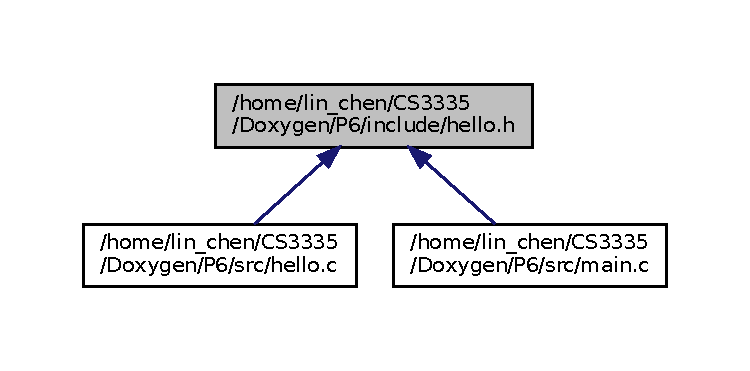
\includegraphics[width=350pt]{hello_8h__dep__incl}
\end{center}
\end{figure}
\subsection*{Functions}
\begin{DoxyCompactItemize}
\item 
char $\ast$ \hyperlink{hello_8h_a568204a6ae5575f8e291eb75fb298207}{hello} ()
\end{DoxyCompactItemize}


\subsection{Function Documentation}
\mbox{\Hypertarget{hello_8h_a568204a6ae5575f8e291eb75fb298207}\label{hello_8h_a568204a6ae5575f8e291eb75fb298207}} 
\index{hello.\+h@{hello.\+h}!hello@{hello}}
\index{hello@{hello}!hello.\+h@{hello.\+h}}
\subsubsection{\texorpdfstring{hello()}{hello()}}
{\footnotesize\ttfamily char$\ast$ hello (\begin{DoxyParamCaption}{ }\end{DoxyParamCaption})}

Return a string \char`\"{}\+Hello World\textbackslash{}n\char`\"{} 
\begin{DoxyParams}[1]{Parameters}
\mbox{\tt out}  & {\em a} & string \\
\hline
\end{DoxyParams}

\hypertarget{util_8h}{}\section{/home/lin\+\_\+chen/\+C\+S3335/\+Doxygen/\+P6/include/util.h File Reference}
\label{util_8h}\index{/home/lin\+\_\+chen/\+C\+S3335/\+Doxygen/\+P6/include/util.\+h@{/home/lin\+\_\+chen/\+C\+S3335/\+Doxygen/\+P6/include/util.\+h}}
This graph shows which files directly or indirectly include this file\+:\nopagebreak
\begin{figure}[H]
\begin{center}
\leavevmode
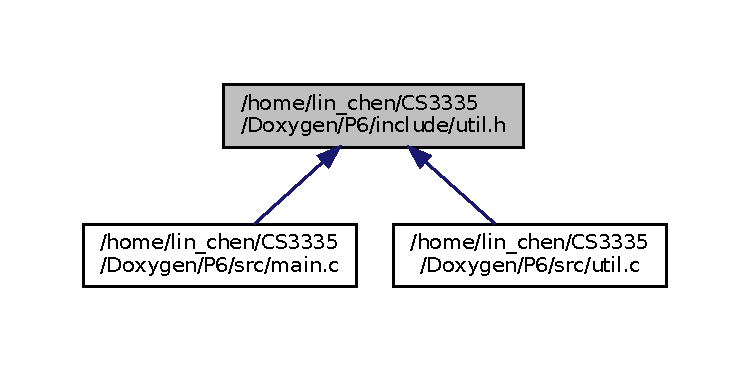
\includegraphics[width=350pt]{util_8h__dep__incl}
\end{center}
\end{figure}
\subsection*{Functions}
\begin{DoxyCompactItemize}
\item 
int \hyperlink{util_8h_a7c825b88e3bac8f6bffadabc109bf190}{double\+Num} (int n)
\end{DoxyCompactItemize}


\subsection{Function Documentation}
\mbox{\Hypertarget{util_8h_a7c825b88e3bac8f6bffadabc109bf190}\label{util_8h_a7c825b88e3bac8f6bffadabc109bf190}} 
\index{util.\+h@{util.\+h}!double\+Num@{double\+Num}}
\index{double\+Num@{double\+Num}!util.\+h@{util.\+h}}
\subsubsection{\texorpdfstring{double\+Num()}{doubleNum()}}
{\footnotesize\ttfamily int double\+Num (\begin{DoxyParamCaption}\item[{int}]{n }\end{DoxyParamCaption})}

Return a double value of an integer 
\begin{DoxyParams}[1]{Parameters}
\mbox{\tt in}  & {\em n} & an integer number \\
\hline
\mbox{\tt out}  & {\em an} & integer number \\
\hline
\end{DoxyParams}

\hypertarget{hello_8c}{}\section{/home/lin\+\_\+chen/\+C\+S3335/\+Doxygen/\+P6/src/hello.c File Reference}
\label{hello_8c}\index{/home/lin\+\_\+chen/\+C\+S3335/\+Doxygen/\+P6/src/hello.\+c@{/home/lin\+\_\+chen/\+C\+S3335/\+Doxygen/\+P6/src/hello.\+c}}
{\ttfamily \#include \char`\"{}hello.\+h\char`\"{}}\newline
Include dependency graph for hello.\+c\+:\nopagebreak
\begin{figure}[H]
\begin{center}
\leavevmode
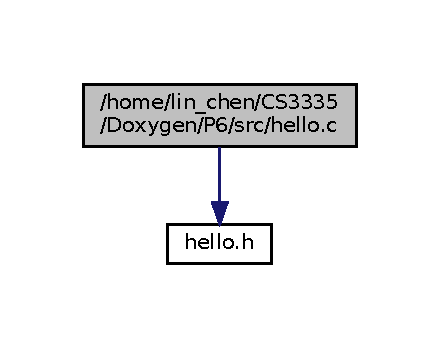
\includegraphics[width=211pt]{hello_8c__incl}
\end{center}
\end{figure}
\subsection*{Functions}
\begin{DoxyCompactItemize}
\item 
char $\ast$ \hyperlink{hello_8c_a568204a6ae5575f8e291eb75fb298207}{hello} ()
\end{DoxyCompactItemize}


\subsection{Function Documentation}
\mbox{\Hypertarget{hello_8c_a568204a6ae5575f8e291eb75fb298207}\label{hello_8c_a568204a6ae5575f8e291eb75fb298207}} 
\index{hello.\+c@{hello.\+c}!hello@{hello}}
\index{hello@{hello}!hello.\+c@{hello.\+c}}
\subsubsection{\texorpdfstring{hello()}{hello()}}
{\footnotesize\ttfamily char$\ast$ hello (\begin{DoxyParamCaption}{ }\end{DoxyParamCaption})}

Return a string \char`\"{}\+Hello World\textbackslash{}n\char`\"{} 
\begin{DoxyParams}[1]{Parameters}
\mbox{\tt out}  & {\em a} & string \\
\hline
\end{DoxyParams}

\hypertarget{main_8c}{}\section{/home/lin\+\_\+chen/\+C\+S3335/\+Doxygen/\+P6/src/main.c File Reference}
\label{main_8c}\index{/home/lin\+\_\+chen/\+C\+S3335/\+Doxygen/\+P6/src/main.\+c@{/home/lin\+\_\+chen/\+C\+S3335/\+Doxygen/\+P6/src/main.\+c}}
{\ttfamily \#include $<$stdio.\+h$>$}\newline
{\ttfamily \#include \char`\"{}hello.\+h\char`\"{}}\newline
{\ttfamily \#include \char`\"{}util.\+h\char`\"{}}\newline
Include dependency graph for main.\+c\+:\nopagebreak
\begin{figure}[H]
\begin{center}
\leavevmode
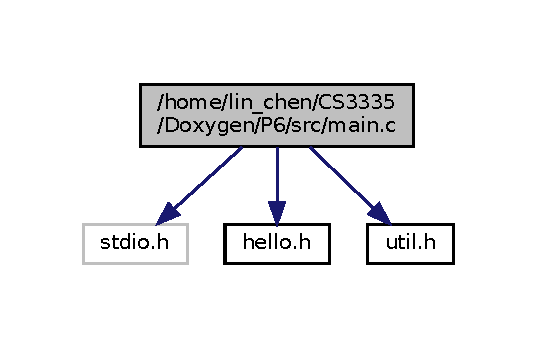
\includegraphics[width=258pt]{main_8c__incl}
\end{center}
\end{figure}
\subsection*{Functions}
\begin{DoxyCompactItemize}
\item 
\mbox{\Hypertarget{main_8c_ae66f6b31b5ad750f1fe042a706a4e3d4}\label{main_8c_ae66f6b31b5ad750f1fe042a706a4e3d4}} 
int {\bfseries main} ()
\end{DoxyCompactItemize}

\hypertarget{util_8c}{}\section{/home/lin\+\_\+chen/\+C\+S3335/\+Doxygen/\+P6/src/util.c File Reference}
\label{util_8c}\index{/home/lin\+\_\+chen/\+C\+S3335/\+Doxygen/\+P6/src/util.\+c@{/home/lin\+\_\+chen/\+C\+S3335/\+Doxygen/\+P6/src/util.\+c}}
{\ttfamily \#include \char`\"{}util.\+h\char`\"{}}\newline
Include dependency graph for util.\+c\+:\nopagebreak
\begin{figure}[H]
\begin{center}
\leavevmode
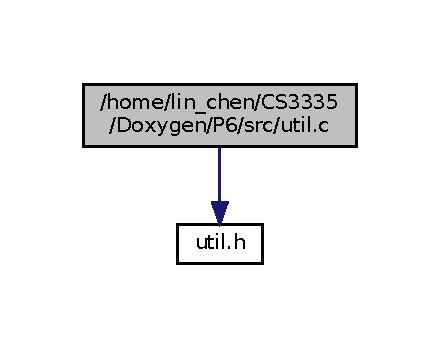
\includegraphics[width=211pt]{util_8c__incl}
\end{center}
\end{figure}
\subsection*{Functions}
\begin{DoxyCompactItemize}
\item 
int \hyperlink{util_8c_a7c825b88e3bac8f6bffadabc109bf190}{double\+Num} (int n)
\end{DoxyCompactItemize}


\subsection{Function Documentation}
\mbox{\Hypertarget{util_8c_a7c825b88e3bac8f6bffadabc109bf190}\label{util_8c_a7c825b88e3bac8f6bffadabc109bf190}} 
\index{util.\+c@{util.\+c}!double\+Num@{double\+Num}}
\index{double\+Num@{double\+Num}!util.\+c@{util.\+c}}
\subsubsection{\texorpdfstring{double\+Num()}{doubleNum()}}
{\footnotesize\ttfamily int double\+Num (\begin{DoxyParamCaption}\item[{int}]{n }\end{DoxyParamCaption})}

Return a double value of an integer 
\begin{DoxyParams}[1]{Parameters}
\mbox{\tt in}  & {\em n} & an integer number \\
\hline
\mbox{\tt out}  & {\em an} & integer number \\
\hline
\end{DoxyParams}

%--- End generated contents ---

% Index
\backmatter
\newpage
\phantomsection
\clearemptydoublepage
\addcontentsline{toc}{chapter}{Index}
\printindex

\end{document}
